% Appendix A

\chapter{Script principal} % Main appendix title

\label{Script principal}

El script principal del proyecto contiene un procesador de líneas de comando que facilita la ejecución de los diferentes casos de uso. Los usos básicos del procesador se detallan a continuación:

\begin{itemize}
    \item Mostrar la ayuda.
\end{itemize}
\begin{verbatim}
$ python src/main.py --help
\end{verbatim}

\begin{itemize}
    \item Jugar un humano contra el bot aleatorio.
\end{itemize}
\begin{verbatim}
$ python src/main.py play --games=<number_of_games> --bot
\end{verbatim}

\begin{itemize}
    \item Jugar un humano contra el agente de Monte Carlo.
\end{itemize}
\begin{verbatim}
$ python src/main.py play --games=<number_of_games> \
    --monte_carlo=<model_file>
\end{verbatim}


\begin{itemize}
    \item Entrenar un nuevo agente de Monte Carlo.
\end{itemize}
\begin{verbatim}
$ python src/main.py train --episodes=<number_of_episodes>
\end{verbatim}

\begin{figure}[htbp]
	\centering
	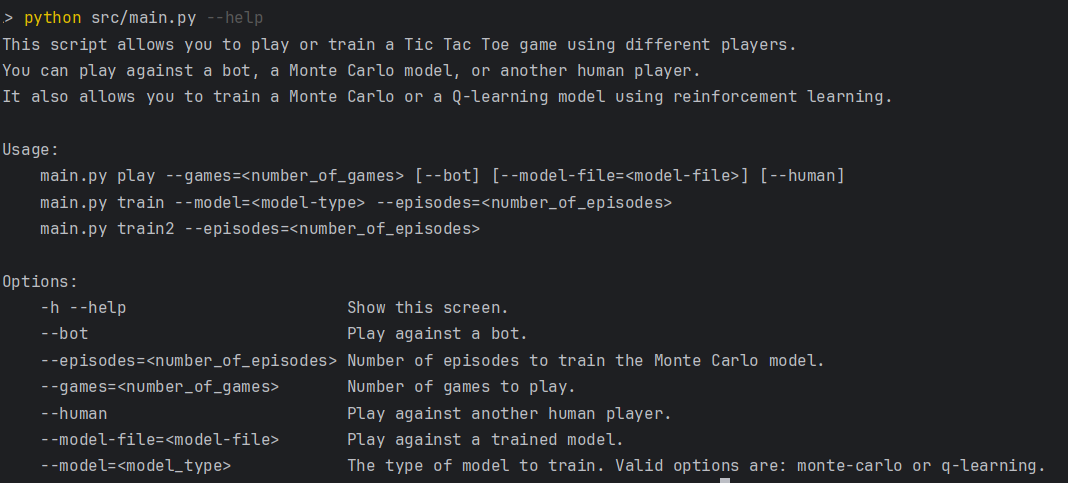
\includegraphics[width=\textwidth]{./Figures/command.png}
	\caption{Uso del script principal por línea de comando.}
	\label{fig:coverage}
\end{figure}